\section{Introduction}
\label{sec:introduction}

% state the learning objective 
The objective of this laboratory assignment is to do analysis on a circuit using the mesh and the nodal method as well as running a simulation using NGspice with the objective of detecting small diferences between the different studies and understand why said differences happens. The circuit can be seen in Figure~\ref{fig:rc}.

In Section~\ref{sec:analysis}, a theoretical analysis of the circuit is
presented. In Section~\ref{sec:simulation}, the circuit is analysed by
simulation, and the results are compared to the theoretical results obtained in
Section~\ref{sec:analysis}. The conclusions of this study are outlined in
Section~\ref{sec:conclusion}.

\begin{figure}[h] \centering
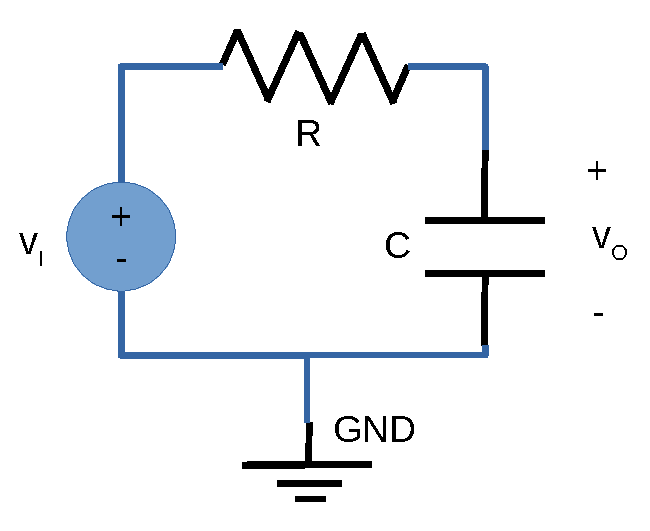
\includegraphics[width=0.5\linewidth]{rc.pdf}
\caption{Circuit with an independent current and voltage source ($V_a$ and $I_d$ respectively) and linear dependent sources ($V_c$-linear current controlled voltage source and $I_b$-linear voltage controlled current source}
\label{fig:rc}
\end{figure}

